\documentclass[10pt]{article}
\usepackage[a4paper,margin=2.4cm]{geometry}
\usepackage[T1]{fontenc}
\usepackage{lmodern}
\usepackage{amsmath,amssymb}
\usepackage{graphicx}
\usepackage{booktabs}
\usepackage{array}
\usepackage[numbers,sort&compress]{natbib}
\usepackage{xcolor}
\usepackage[colorlinks=true,linkcolor=blue!50!black,citecolor=blue!50!black,urlcolor=blue!50!black]{hyperref}
\usepackage{caption}
\captionsetup{font=small,labelfont=bf}

\newcommand{\bplMAE}{0.019}
\newcommand{\swtMAE}{0.027}
\newcommand{\ifboMAE}{0.086}
\newcommand{\bplHB}{0.124}
\newcommand{\bplFT}{0.089}
\newcommand{\swtHB}{0.116}
\newcommand{\swtFT}{0.094}
\newcommand{\ifboHB}{0.071}
\newcommand{\ifboFT}{0.083}
\newcommand{\realHB}{0.155}
\newcommand{\realFT}{0.112}
\newcommand{\fitHB}{0.140}
\newcommand{\fitFT}{0.089}
\newcommand{\fitMAE}{0.014}
\newcommand{\bplAUC}{0.88}
\newcommand{\swtAUC}{0.89}
\newcommand{\ifboAUC}{0.91}
\newcommand{\bplPrec}{0.71}
\newcommand{\bplRec}{0.79}
\newcommand{\swtPrec}{0.64}
\newcommand{\swtRec}{0.76}
\newcommand{\ifboPrec}{0.61}
\newcommand{\ifboRec}{0.72}
\newcommand{\bplRho}{0.70}
\newcommand{\realRho}{0.77}
\newcommand{\bplSpeed}{0.51}
\newcommand{\realSpeed}{0.73}
\newcommand{\ifboSpeed}{0.22}
\newcommand{\bplNinety}{-1.50}
\newcommand{\realNinety}{-1.10}
\newcommand{\bplOver}{0.01}
\newcommand{\realOver}{0.04}
\newcommand{\bplNoise}{0.04}
\newcommand{\realNoise}{0.15}
\newcommand{\bplFinal}{0.55}
\newcommand{\realFinal}{0.48}
\newcommand{\bplVersion}{16}

\newcommand{\bpl}{\textsf{bpl}}

\title{Broken Power Laws on the Right Scale:\\A Data-Driven Prior of Learning Curves for Freeze-Thaw HPO}
\author{Authors withheld (draft)}
\date{\today}

\begin{document}
\maketitle

\begin{abstract}
Freeze-thaw hyperparameter optimisation (HPO) decides from partial learning curves which training runs to
continue. Its strongest recent methods are trained on synthetic tasks from a hand-designed prior. We build such a
prior from data. From about 760 real HPO tasks we establish what their curves are (validation losses or bounded
error rates, under constant, decaying or cosine learning-rate schedules) and which known phenomena they show:
power-law decline after a plateau, a floor, schedule effects, overfitting and instabilities, divergence, and
heteroscedastic heavy-tailed noise. Comparing loss scales and time axes, curves are best described as broken power
laws on the scale $\log(\text{loss} - \text{floor})$, in time measured as optimiser progress: the cumulative
learning rate of the configuration's schedule, warped by the learning rate. On this scale one component explains
84--94\% of the variation between the curves of a task. The resulting generator, \bpl{}, samples search spaces
with a learning-rate and schedule dimension and a validation curve for every configuration, in raw units. On
held-back task families, existing HPO algorithms behave on \bpl{} tasks much closer to real tasks than on tasks
from the prior used to train FT-PFN: the mean difference of regrets from real is \bplMAE{} (FT-PFN prior:
\ifboMAE{}), and Hyperband gains \bplHB{} over random search (real \realHB{}; FT-PFN prior \ifboHB{}). We also
report what \bpl{} does not yet reproduce: curves level off too early, late noise is too small, rising curves are
too rare, and landscapes are less predictable from the configuration than real ones.
\end{abstract}

\section{Introduction}

Learning-curve-based HPO saves compute by training many configurations briefly and only the promising ones to
the end~\cite{swersky2014freeze,li2018hyperband,wistuba2022supervising}. Its decisions rest on a model of how a
partial curve continues and how the curves of different configurations relate. Prior-data fitted networks
(PFNs)~\cite{muller2022transformers} learn such a model entirely from synthetic data: LC-PFN extrapolates single
curves~\cite{adriaensen2023efficient}, and FT-PFN, the surrogate of ifBO~\cite{rakotoarison2024incontext}, models
whole tasks. What these models believe about learning curves comes from the prior that generated their training
data. In ifBO that prior is hand-designed: curves are mixtures of parametric saturating families, and
configurations act through a random neural network.

We build the prior from data. We ask what real learning curves of HPO tasks are, how they vary within and between
tasks, how the configuration shapes them, and what their noise looks like. Each answer becomes a part of the
generator. We test the generator on held-back task families, with statistics of real data and with existing HPO
algorithms. No HPO model is trained in this work.

\paragraph{Contributions.}
\begin{enumerate}
  \item A description of real HPO learning curves aimed at generative modelling: their semantics per source, a
    check of known phenomena against the data, and a comparison of representations (loss scale $\times$ time axis).
  \item \bpl{}, a generator of synthetic HPO tasks: broken power laws on the log-excess scale in schedule-aware
    progress time, with learning-rate and schedule dimensions, rising curves, divergence, dead configurations and
    heteroscedastic heavy-tailed noise.
  \item An evaluation on held-back task families that separates curve shape, noise, landscape and HPO behaviour,
    with the ifBO prior as baseline.
\end{enumerate}

\section{Related work}

\paragraph{Shapes of learning curves.} Surveys~\cite{viering2022shape,mohr2022learning} document power-law,
exponential and more complex shapes, including plateaus, peaks and non-monotone curves. Curve extrapolation
combines parametric families~\cite{domhan2015speeding} or learns them with Bayesian neural
networks~\cite{klein2017learning} and PFNs~\cite{adriaensen2023efficient}.
\paragraph{Scaling laws.} Loss falls as a power law in data, model size and compute
\cite{hestness2017deep,kaplan2020scaling}, so that $\log(\text{loss} - \text{floor})$ is linear in log-time
after an initial plateau; broken power laws~\cite{caballero2023broken} join a plateau and one or more power-law
segments smoothly. Tissue et al.~\cite{tissue2024scaling} describe the loss under a learning-rate schedule with the
cumulative learning rate (``forward area'') and an annealing term. We test both ingredients on HPO curves.
\paragraph{Within-task structure.} Modelling a family of curves as one shape with per-curve shifts and scales is
old in statistics (self-modelling regression~\cite{lawton1972self}, SITAR~\cite{cole2010sitar}); functional
principal components~\cite{ramsay2005functional} measure how many directions the curves of a task vary in.
\paragraph{Priors for freeze-thaw HPO.} Freeze-thaw BO~\cite{swersky2014freeze} assumed exponentially decaying
curves under a GP; DyHPO~\cite{wistuba2022supervising} learns a deep kernel over configurations and budgets; ifBO's
FT-PFN~\cite{rakotoarison2024incontext} is trained on a hand-designed prior, our baseline.

\section{Data}
\label{sec:data}

\paragraph{Sources and semantics.} A task is a search space, a set of configurations (up to 1000) and for each one
a learning curve. Table~\ref{tab:data} lists what the curves are. All are \emph{validation} metrics; three
sources are unbounded losses and three are bounded error rates. Values $\le 0$ occur in 21\% of TaskSet tasks
(negative log-likelihoods of density models, quadratic objectives), which matters for the choice of scale
(Section~\ref{sec:representation}). TaskSet's optimiser families define the learning-rate schedule as
hyperparameters; JAHS-Bench-201 and NAS-Bench-201 use one fixed cosine schedule over the full budget.

\begin{table}[t]
\centering\small
\caption{What the curves are, per source. The ``tasks'' column counts fit / select tasks (see below).}
\label{tab:data}
\begin{tabular}{p{2.2cm}p{3.2cm}lp{1.4cm}p{5.0cm}}
\toprule
source & metric (all validation) & tasks & time axis & learning-rate schedule \\
\midrule
TaskSet~\cite{metz2020using} & loss, unbounded; $\le 0$ in 21\% of tasks & 400 / 150 & 50 points over 10k steps, plus step 0 &
  hyperparameters: constant (adam1p, adam4p), linear and exponential decay (adam6p, adam8p), warm-up + constant + cosine (nadamw) \\
JAHS-Bench-201~\cite{bansal2022jahs} & error (\%), bounded & 81 / 0 & 200 epochs & fixed cosine to 0 \\
NAS-Bench-201~\cite{dong2020nasbench201} & error (fraction), bounded & 3 / 0 & 200 epochs & fixed cosine to 0 \\
QuickTune~\cite{pineda2024quicktune} & error (\%), bounded; 0 reached in 11\% & 86 / 0 & $\le$ 50 epochs & a scheduler hyperparameter (not modelled) \\
FCNet~\cite{klein2019tabular} & MSE, unbounded & 0 / 4 & 100 epochs & constant or cosine (hyperparameter) \\
bbomix~\cite{salinas2022synetune} & loss, unbounded & 0 / 35 & 300 epochs & none recorded \\
\bottomrule
\end{tabular}
\end{table}

\paragraph{Splits.} Tasks are split by family so that whole families are held back. The \emph{fit} split (570 tasks)
is used to build the generator; the \emph{select} split (189 tasks: TaskSet families char, conv, rnn, Associative and
Copy, FCNet, bbomix) only for evaluation. All numbers in Section~\ref{sec:results} are measured on select tasks; all
analyses in Sections~\ref{sec:phenomena} and~\ref{sec:representation} on fit tasks. LCBench~\cite{zimmer2021autopytorch},
PD1~\cite{wang2024pretrained} and TaskSet's FixedTextRNNClassification tasks are the test benchmarks of FT-PFN; they
are not used in any way.

\section{Known phenomena in the data}
\label{sec:phenomena}

Table~\ref{tab:phenomena} lists what is known about training curves, what the fit data shows, and whether \bpl{}
produces it.

\begin{table}[t]
\centering\small
\caption{Known phenomena of training curves: what the fit data shows, and whether \bpl{} produces it.}
\label{tab:phenomena}
\begin{tabular}{p{3.7cm}p{6.8cm}p{4.0cm}}
\toprule
phenomenon & in the data & in \bpl{} \\
\midrule
plateau, then power-law decline & everywhere; a logistic in log-time with a floor fits TaskSet curves to noise level & yes: broken power law \\
irreducible floor per config & yes; final values differ between configs that have converged & yes: floor offset $d$ \\
learning rate as a time warp & curve time scale $\propto \eta^{-\kappa}$, $\kappa \approx 0.15$ on TaskSet (quartiles 0.07--0.27) & yes \\
schedule (decay, warm-up, cosine) & decayed configs are predicted better in cumulative-learning-rate time (Table~\ref{tab:schedule}) & yes, for TaskSet families and fixed cosine \\
annealing drop at the end of a decay & an annealing term~\cite{tissue2024scaling} does not improve predictions from partial curves & no \\
overfitting (validation rises, training falls) & 3.6\% of live TaskSet curves rise after their minimum, 11\% on bbomix, $\approx 0$ under cosine annealing; in TaskSet mostly with rising training loss too (instability), classic overfitting in a few families (73\% of rising curves of image convnets) & partly: one rise term for both; too rare (Section~\ref{sec:results}) \\
divergence & sharp region at high learning rates, predictable from the config (AUC 0.99) & yes \\
no learning (dead) & sharp region at low learning rates & yes \\
noise grows with the loss level & error rates: residual sd $\propto$ excess$^{1.3\text{--}1.4}$; TaskSet losses: no growth & yes, per task exponent \\
heavy-tailed noise & excess kurtosis 0.5--8 per source & yes: Student-$t$ \\
seed-to-seed variation & 24--37\% of final-value variance among the best 10\% of configs & no (one seed per config) \\
training vs.\ validation gap & training curves only in TaskSet & no (validation only) \\
budget-dependent schedule horizon & benchmarks fix the horizon; a shorter run is a prefix of a long one & no \\
\bottomrule
\end{tabular}
\end{table}

\section{The representation}
\label{sec:representation}

A generator needs a scale on which configurations and noise act, and a time axis. We compared the standard choices
on 226 fit tasks.

\paragraph{Curve form.} A broken power law,
\begin{equation}
  y(x) = L + d + \frac{A}{1 + (x/\tau)^{a}},
  \label{eq:bpl}
\end{equation}
has a plateau at $L + d + A$, a knee at $\tau$, and then a power-law decline $y - L - d \propto x^{-a}$ towards a
floor $L + d$, where $L$ is the task's floor and $d \ge 0$ the configuration's own offset above it. Plain power laws
fit HPO curves poorly because these curves have plateaus; Eq.~\eqref{eq:bpl} fits them to about the noise level
(median RMSE on the log-excess scale 0.019 for TaskSet, 0.035 for QuickTune, 0.19 for the noisy error rates near
their floor on JAHS and NAS-Bench-201).

\paragraph{Loss scale.} Plain $\log y$ is impossible for the 21\% of TaskSet tasks with values $\le 0$. We use the
log-excess scale $v = \log(y - L)$ with a task floor $L$ = task minimum $- 0.02 \times$ task range, and compare it
with the linear scale (Table~\ref{tab:repr}; a floor at 0.1 of the range gives the same ranking).
\begin{itemize}
  \item \emph{Structure within a task}: the share of variance between a task's curves explained by the first
    functional principal component is higher on the log-excess scale on every source (84--94\% vs.\ 81--91\%);
    two components explain 89--98\%. The curves of a task are close to ``one shared curve plus one
    configuration-specific direction'', which keeps their order over time.
  \item \emph{Partial-curve prediction} (what freeze-thaw needs): Eq.~\eqref{eq:bpl} fitted on the first 40\% of a
    curve, final value predicted. The log-excess scale ranks finals better on TaskSet, QuickTune and JAHS and has a
    lower error on TaskSet and JAHS. No curve model ranks finals better than the current value itself, a strong
    baseline at 40\% of the budget; the comparison is between scales.
  \item \emph{Noise}: the slope $k$ of log residual size on log excess is 1.3--1.4 on error-rate sources
    (multiplicative noise) and near 0 on TaskSet and QuickTune (additive). Neither scale makes the noise
    homoscedastic everywhere, so the generator uses $\text{sd} \propto \text{excess}^{k}$ with $k$ fitted per task.
\end{itemize}

\begin{table}[t]
\centering\small
\caption{Loss scale, compared on fit tasks (medians over tasks; bold: the better scale). Predictions use the first
40\% of each curve. ``Current value'': ranking finals by the value at 40\%, for scale. Error of finals: median
absolute error as a share of the task range. Noise slope $k$: residual sd $\propto$ excess$^k$. NAS-Bench-201 has
only 3 fit tasks.}
\label{tab:repr}
\resizebox{\linewidth}{!}{\begin{tabular}{lrrrrrrrr}
\toprule
 & tasks & \multicolumn{2}{c}{variance explained by 1 component $\uparrow$} & \multicolumn{3}{c}{rank corr.\ of predicted finals $\uparrow$} & error of finals $\downarrow$ & noise slope \\
\cmidrule(lr){3-4}\cmidrule(lr){5-7}\cmidrule(lr){8-8}
source & & linear & log-excess & linear & log-excess & current value & linear / log-excess & $k$ \\
\midrule
TaskSet & 144 & 0.908 & \textbf{0.938} & 0.80 & \textbf{0.86} & 0.94 & 0.042 / 0.032 & -0.14 \\
QuickTune & 39 & 0.898 & \textbf{0.924} & 0.81 & \textbf{0.85} & 0.91 & 0.058 / 0.060 & 0.10 \\
JAHS & 40 & 0.809 & \textbf{0.840} & 0.37 & \textbf{0.57} & 0.60 & 0.061 / 0.045 & 1.44 \\
NB201 & 3 & 0.877 & \textbf{0.897} & \textbf{0.52} & 0.40 & 0.87 & 0.176 / 0.180 & 1.29 \\
\bottomrule
\end{tabular}
}
\end{table}

\paragraph{Time axis.} Log-time is the standard axis of power laws. What it leaves out is the schedule: a
configuration whose learning rate decays to zero makes little progress late in training however many steps it
takes. We measure time as optimiser progress,
\begin{equation}
  x = (\eta/\eta_\text{ref})^{\kappa}\; S_1(t)/T_\text{total}, \qquad S_1(t) = \textstyle\sum_{s \le t} m(s),
  \label{eq:progress}
\end{equation}
where $m(s)$ is the schedule's learning-rate multiplier (1 for constant schedules), $\eta$ the base learning rate
and $\kappa$ a per-task exponent. For decayed configurations, finals are predicted better from partial curves in
progress time than in step time; for constant schedules nothing changes (Table~\ref{tab:schedule}). The learning
rate acts as a partial time warp: from the slope of the time to 50\% progress on the log learning rate, the median
over TaskSet tasks is $\kappa = 0.15$ (quartiles 0.07--0.27), far from a full warp ($\kappa = 1$). The annealing term
of~\cite{tissue2024scaling} does not improve predictions from partial curves and is not used.

\begin{table}[t]
\centering\small
\caption{Time axis, compared on TaskSet fit tasks with schedule hyperparameters: Eq.~\eqref{eq:bpl} fitted on the first
40\% of each curve on the log-excess scale, in step time or in progress time $S_1$ (Eq.~\ref{eq:progress}). Bold: the
better axis (none if equal). Error of finals as a share of the task range. nadamw with an (almost) constant schedule
has too few curves per task to rank.}
\label{tab:schedule}
\begin{tabular}{llrrrrr}
\toprule
 & & & \multicolumn{2}{c}{rank corr.\ of predicted finals $\uparrow$} & \multicolumn{2}{c}{error of finals $\downarrow$} \\
\cmidrule(lr){4-5}\cmidrule(lr){6-7}
learning rate at the end & family & curves & step time & progress time & step time & progress time \\
\midrule
$<$ 0.5 $\times$ initial & adam6p & 1120 & 0.951 & \textbf{0.964} & 0.017 & \textbf{0.014} \\
 & adam8p & 906 & 0.896 & \textbf{0.933} & 0.016 & \textbf{0.013} \\
 & nadamw & 2223 & 0.855 & \textbf{0.880} & 0.021 & \textbf{0.018} \\
$\ge$ 0.9 $\times$ initial & adam6p & 494 & 0.888 & 0.888 & 0.022 & \textbf{0.022} \\
 & adam8p & 340 & 0.871 & 0.871 & \textbf{0.019} & 0.020 \\
\bottomrule
\end{tabular}

\end{table}

\paragraph{What makes curve speed depend on the configuration.} On TaskSet, the time a curve takes to make half its
progress is predictable from the configuration ($R^2$ 0.90), mostly through the learning rate (0.58 from it alone,
$-0.15$ without it). On JAHS-Bench-201 it is also predictable (0.74), but not from the learning rate (0.00): there
architecture and data augmentation drive speed. A generator must therefore let the configuration set the shape of
a curve and not only its final value, and the learning rate cannot be the only driver.

\begin{figure}[t]
  \centering
  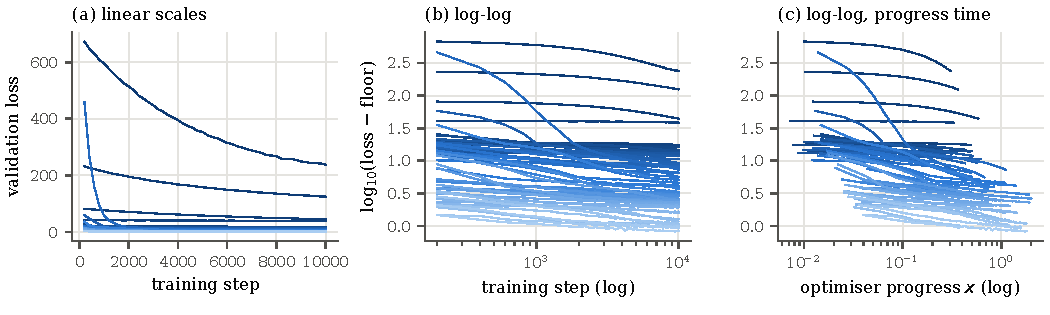
\includegraphics[width=\linewidth]{figures/bpl_representation.pdf}
  \caption{One real TaskSet task (a word-level RNN language model, adam6p with decaying schedules; 60 live
  configurations, colour: final value, dark = good). (a) Linear loss over steps: a few configurations dominate the
  scale. (b) $\log_{10}(\text{loss} - L)$ over log steps: plateaus followed by near-linear declines. (c) The same
  over optimiser progress (Eq.~\ref{eq:progress}): configurations whose learning rate decays end at less progress.}
  \label{fig:repr}
\end{figure}

\section{The generator \bpl{}}
\label{sec:model}

\begin{figure}[t]
  \centering
  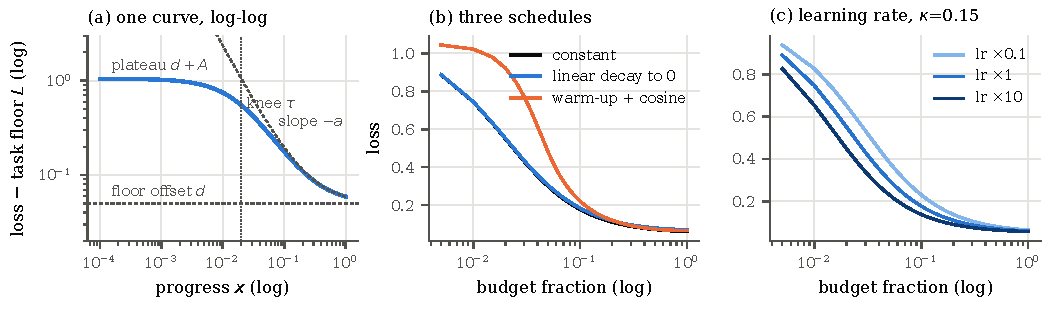
\includegraphics[width=\linewidth]{figures/bpl_model.pdf}
  \caption{The curve model. (a) Eq.~\eqref{eq:bpl} on log-log axes: plateau, knee, power-law segment and floor
  offset. (b) The same parameters under three schedules over the budget: a warm-up delays progress; a decay slows
  it late (in progress time, decay can only slow a curve; the extra drop that annealing often causes is not
  modelled). (c) The learning rate shifts the curve in time by a factor $\eta^{\kappa}$.}
  \label{fig:model}
\end{figure}

\paragraph{Records.} For each fit task we fit Eq.~\eqref{eq:bpl} to every live curve on the log-excess scale in
progress time (least squares on $v$; for TaskSet the step-0 value, before training, is kept as the task's start
level). A task becomes a \emph{record}: the floor $L$ and start level; the joint distribution of per-curve parameters
$(\log d, \log A, \log \tau, \log a)$, with $\tau$ in progress units so that learning rate and schedule are factored
out; $\kappa$; the learning-rate range of live configurations and, for TaskSet, the real distributions of the
schedule hyperparameters; the relation between each parameter and the learning rate; the share, onset and size of
rising curves; dead and diverged shares, dead level and divergence times; noise level, its profile over the budget,
excess exponent $k$ and tail weight. 556 of 570 fit tasks give a record.

\paragraph{Generating a task.} One draw proceeds as follows (Figure~\ref{fig:anatomy}).
\begin{enumerate}
  \item \textbf{Search space.} Pick a record and take its number of hyperparameters $d \le 10$; configurations are
    uniform in $[0,1]^d$. Dimension 0 is the log learning rate over the record's range. For TaskSet records the next
    dimensions are the schedule hyperparameters of the record's optimiser family, mapped to their real marginals;
    the remaining dimensions are generic.
  \item \textbf{Progress time.} Each configuration's progress $x(t)$ follows from its learning rate and schedule by
    Eq.~\eqref{eq:progress}.
  \item \textbf{Parameters.} Seven Gaussian-process fields with a random Mat\'ern-5/2 kernel (random relevance per
    dimension) are drawn over the configurations. Four of them give normal scores for the four curve parameters,
    correlated like the record's real parameters (a Gaussian copula); each score is shifted by the record's real
    conditional mean given the log learning rate, and mapped through the real marginal. The field of the floor
    offset is mixed with a rough companion so that the landscape is as predictable from the configuration as the
    record's real one. Parameters thus vary smoothly over the search space, which keeps the early rankings of
    configurations consistent, as in real tasks.
  \item \textbf{Start consistency (TaskSet).} All TaskSet runs start from the same initial loss. Amplitude and floor
    offset are capped so that no live curve starts above it.
  \item \textbf{Rising curves.} A share of the configurations (from the record) rises after an onset by a relative
    amount drawn from the record.
  \item \textbf{Dead and diverged.} Dead configurations sit at the low end of the learning-rate axis and diverged ones
    at the high end, mixed with two further fields; dead curves stay at the record's dead level, diverged curves
    jump to a high value at a divergence time drawn from the record.
  \item \textbf{Noise.} Student-$t$ noise with the record's tail weight, level and time profile, scaled by
    $(\text{excess}/\text{median excess})^{k}$.
\end{enumerate}
Output is in the record's raw units, labelled as loss or error rate; error rates are clipped to their range. No real
curve is replayed: what is reused from real tasks are distributions (of parameters, classes, noise) and their
relations to the learning rate.

\begin{figure}[t]
  \centering
  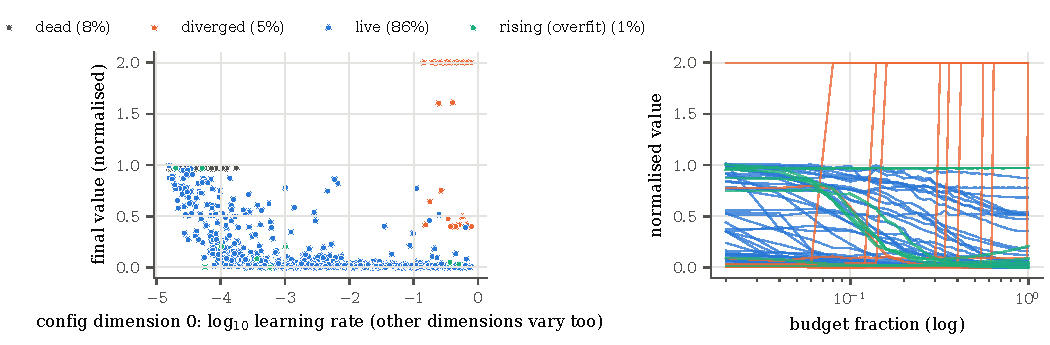
\includegraphics[width=\linewidth]{figures/bpl_anatomy.pdf}
  \caption{One generated task from a TaskSet record. Left: final value against the learning rate (configuration
  dimension 0; the other dimensions, including the schedule, also vary). Dead configurations sit at the low end,
  diverged ones at the high end. Right: a sample of its curves by class.}
  \label{fig:anatomy}
\end{figure}

\section{Evaluation}
\label{sec:protocol}

We compare \bpl{} with real held-back tasks and with the prior used to train FT-PFN (``ifBO prior''), each with as
many generated tasks as real ones. Values are normalised per task for the statistics, $z = (y - y_\text{best}) /
(y_\text{ref} - y_\text{best})$ with $y_\text{ref}$ the 90th percentile of first values (0 = the task's best, 1 = a
typical start; capped at 2). A curve is \emph{dead} if it never falls below 0.9, \emph{diverged} if it reaches the
cap, and \emph{live} otherwise. Each statistic is computed per task and summarised by its median over the 189 select
tasks.
\begin{itemize}
  \item \textbf{Curves.} On live curves resampled to 40 points in log-time: the log budget fraction at which a curve
    has made 50\% and 90\% of its progress; the progress made in the last 20\% of the budget; the share of curves
    that rise after their minimum; the final value. A classifier two-sample test~\cite{lopezpaz2017revisiting}
    (cross-validated AUC of boosted trees telling real from generated curves; 0.5 = it cannot) and $k$-NN precision
    and recall~\cite{kynkaanniemi2019improved} in an 8-dimensional PCA embedding.
  \item \textbf{Noise.} Residuals from a smoothed curve: excess kurtosis, and residual spread in the last third
    relative to the first third.
  \item \textbf{Landscape.} The rank correlation between final values and the predictions of boosted trees trained
    on 200 configurations; the share of configurations within 0.05 of the best; local optima on a
    10-nearest-neighbour graph relative to a random permutation of the same values (1 = as rugged as noise); and the
    cross-validated $R^2$ of predicting a live curve's time to 50\% progress from its configuration.
  \item \textbf{HPO behaviour.} Random search, Hyperband~\cite{li2018hyperband} ($\eta = 3$) and a freeze-thaw
    heuristic with budgets of 1--20 full trainings. Regret is the rank of the incumbent's final value among all
    configurations (0 = best). We report the mean absolute difference of the mean regrets from the real ones over
    algorithms and budgets, and the \emph{gain} of Hyperband and freeze-thaw over random search (regret difference
    averaged over budgets). Each generator is run with three generation seeds; the standard error of a gain over
    tasks is about 0.01.
\end{itemize}

\section{Results}
\label{sec:results}

\begin{figure}[t]
  \centering
  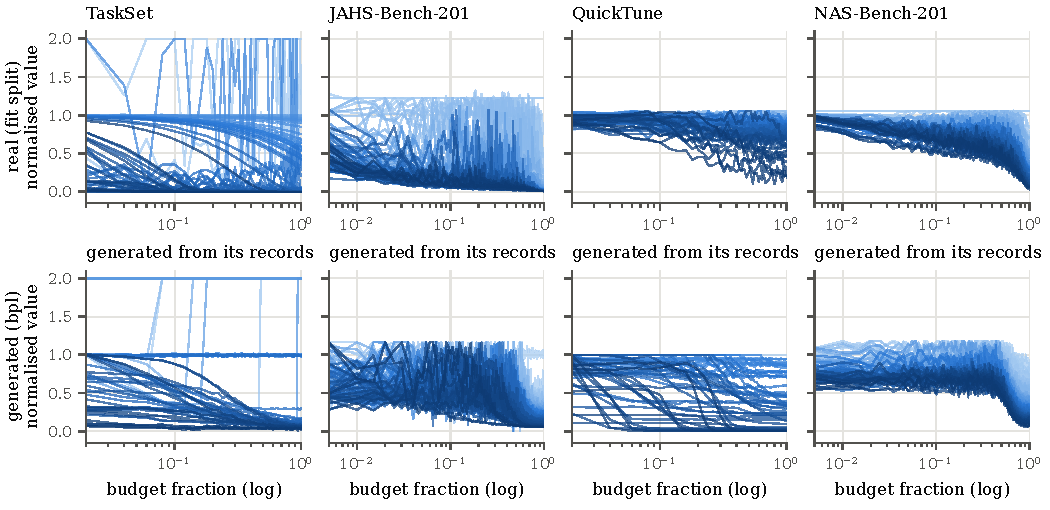
\includegraphics[width=\linewidth]{figures/bpl_examples.pdf}
  \caption{Top: real tasks (fit split, 80 random configurations; TaskSet without the step-0 point). Bottom: tasks
  generated by \bpl{} from records of the same source (configurations, parameter fields and curves are new). Colour:
  final value (dark = good). Normalised values; $x$-axis logarithmic.}
  \label{fig:examples}
\end{figure}

\begin{table}[t]
  \centering
  \small
  \caption{\bpl{} and the ifBO prior compared with real data on the select split (189 held-back real tasks; medians
  over tasks). The reference column is real data; the last column says which direction is better; the better
  generator per row is bold. HPO rows: mean over three generation seeds.}
  \label{tab:compare}
  \resizebox{\linewidth}{!}{\begin{tabular}{llrrrl}
\toprule
 & statistic & \textbf{real (reference)} & ifBO prior & bpl & better \\
\midrule
Curves & time to 50\% of progress (log budget fraction) & -2.708 & -1.806 & \textbf{-2.809} & closer to real \\
Curves & time to 90\% of progress (log budget fraction) & -1.103 & -0.602 & \textbf{-1.505} & closer to real \\
Curves & progress in the last 20\% of the budget & 0.029 & 0.092 & \textbf{0.015} & closer to real \\
Curves & share of curves rising after their minimum & 0.039 & 0.124 & \textbf{0.014} & closer to real \\
Curves & final value (normalised) & 0.479 & 0.683 & \textbf{0.555} & closer to real \\
Curves & classifier telling real from generated (AUC, 0.5 = cannot) & -- & 0.911 & \textbf{0.883} & lower \\
Curves & generated curves that look real (precision) & -- & 0.613 & \textbf{0.712} & higher \\
Curves & real curves the generator can produce (recall) & -- & 0.721 & \textbf{0.793} & higher \\
\midrule
Noise & excess kurtosis of residuals & 23.3 & 0.140 & \textbf{25.6} & closer to real \\
Noise & residual spread, last third / first third & 0.152 & 0.810 & \textbf{0.045} & closer to real \\
\midrule
Landscape & final value predictable from config (rank corr.) & 0.771 & \textbf{0.734} & 0.696 & closer to real \\
Landscape & share of configs within 0.05 of the best & 0.136 & 0.013 & \textbf{0.090} & closer to real \\
Landscape & local optima relative to random (1 = random) & 0.461 & \textbf{0.526} & 0.604 & closer to real \\
Landscape & curve speed predictable from config ($R^2$) & 0.730 & 0.218 & \textbf{0.511} & closer to real \\
\midrule
HPO & Hyperband gain over random search & 0.155 & 0.071 & \textbf{0.124} & closer to real \\
HPO & freeze-thaw gain over random search & 0.112 & 0.083 & \textbf{0.089} & closer to real \\
HPO & regret difference from real (mean abs.) & 0.000 & 0.086 & \textbf{0.019} & lower \\
\bottomrule
\end{tabular}
}
\end{table}

\begin{table}[t]
  \centering
  \small
  \caption{HPO behaviour: mean over three generation seeds ($\pm$ standard deviation over seeds). ``Real fit tasks''
  runs the same algorithms on the real tasks \bpl{} was built from: a generator that copied them exactly would score
  about there. Bold: the better generator per column.}
  \label{tab:hpo}
  \begin{tabular}{lrrrr}
\toprule
 & seeds & regret difference from real $\downarrow$ & Hyperband gain & freeze-thaw gain \\
\midrule
\textbf{real select tasks (reference)} & -- & 0.000 & 0.155 & 0.112 \\
real fit tasks & -- & 0.014 & 0.140 & 0.089 \\
\midrule
ifBO prior & 3 & 0.086 {\scriptsize$\pm$0.006} & 0.071 {\scriptsize$\pm$0.007} & 0.083 {\scriptsize$\pm$0.007} \\
bpl & 3 & \textbf{0.019} {\scriptsize$\pm$0.003} & \textbf{0.124} {\scriptsize$\pm$0.017} & \textbf{0.089} {\scriptsize$\pm$0.006} \\
\midrule
better & & lower & closer to 0.155 & closer to 0.112 \\
\bottomrule
\end{tabular}

\end{table}

\paragraph{HPO behaviour.} This is what a prior for freeze-thaw methods must get right (Table~\ref{tab:hpo},
Figure~\ref{fig:hpo}). On ifBO-prior tasks Hyperband gains only \ifboHB{} over random search (real: \realHB{}),
and regrets stay high at large budgets for all algorithms; the mean difference of regrets from real is \ifboMAE{}.
On \bpl{} tasks it is \bplMAE{}, and Hyperband gains \bplHB{}. The freeze-thaw heuristic gains \bplFT{} on \bpl{}
tasks and \ifboFT{} on ifBO-prior tasks, against \realFT{} on real held-back tasks. The real fit tasks themselves give
only \fitFT{}: the held-back families are easier for early stopping than the families \bpl{} was built from, so part
of this gap cannot be closed by a generator fitted on the fit split.

\begin{figure}[t]
  \centering
  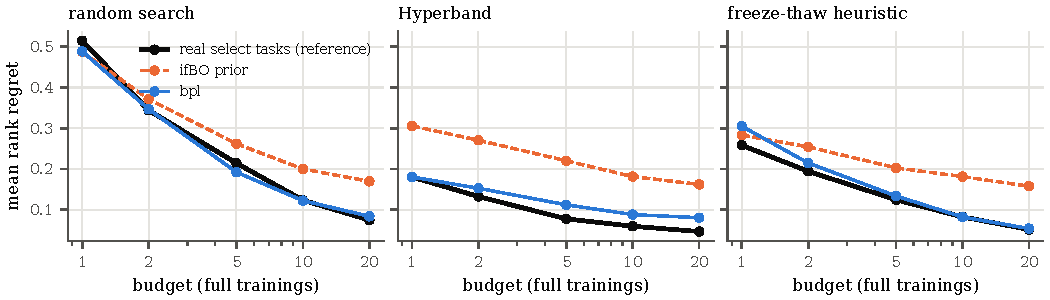
\includegraphics[width=\linewidth]{figures/res_hpo.pdf}
  \caption{Mean rank regret (lower is better) of three HPO algorithms on real select tasks and on generated tasks
  (three generation seeds each).}
  \label{fig:hpo}
\end{figure}

\paragraph{Curves.} Generated curves lie closer to the real ones than ifBO-prior curves by $k$-NN precision and
recall (\bplPrec{} and \bplRec{}; ifBO: \ifboPrec{} and \ifboRec{}); a classifier on single curves still separates
them (AUC \bplAUC{}; ifBO \ifboAUC{}). Two curve statistics are clearly off. Curves level off too early (time to
90\% of progress \bplNinety{} vs.\ \realNinety{} in log budget fraction, with about half the real progress in the
last 20\% of the budget); real configurations replayed with their own fitted curves are also early, so part of the cause is that
Eq.~\eqref{eq:bpl} underfits slow late improvement. And too few curves rise after their minimum (\bplOver{} vs.\ \realOver{}): the held-back families rise
more often than the fit families (bbomix 11\%), and \bpl{} draws the share from fit records. ifBO-prior curves make
their progress much too late and rise far too often.

\paragraph{Noise.} \bpl{} reproduces the heavy tails of real residuals (Table~\ref{tab:compare}); the ifBO prior's
Gaussian noise has none. Late noise is too small relative to early noise (ratio \bplNoise{} vs.\ \realNoise{}):
generated curves have a sharper first step and about 35\% too little noise in the early-middle phase. The ifBO prior
errs in the other direction (0.81).

\paragraph{Landscapes.} \bpl{} produces near-optimal regions of realistic size (ifBO tasks have almost none) and curve
speed that depends on the configuration ($R^2$ \bplSpeed{} vs.\ real \realSpeed{}; ifBO \ifboSpeed{}). Its landscapes
are less predictable from the configuration than real ones (\bplRho{} vs.\ \realRho{}) and more rugged; on these two
statistics the ifBO prior is closer to real.

\section{Limitations}

\begin{itemize}
  \item \textbf{Timing and late noise.} Curves level off too early and late noise is too small; both matter for
    freeze-thaw methods, which extrapolate from early segments.
  \item \textbf{Rising curves} are too rare, and overfitting and instabilities share one rise term; the training
    curve is not generated, so a method cannot use the train/validation gap.
  \item \textbf{Landscapes} are less predictable from the configuration and more rugged than real ones.
  \item \textbf{Freeze-thaw gain} is below the real one on held-back families (\bplFT{} vs.\ \realFT{}), though equal to
    that of the real fit tasks.
  \item \textbf{Schedules} are represented only for TaskSet's families and fixed cosine schedules; QuickTune's
    schedulers are treated as constant, and a budget-dependent horizon (a cosine schedule set for the run's own
    length) is not modelled.
  \item \textbf{NAS-Bench-201-like tasks}: diverged configurations are clipped at 100\% error (real collapse sits near
    chance level), and first values are spread far wider than in real tasks.
  \item \textbf{One seed per configuration}, although seed noise accounts for a quarter to a third of the
    final-value variance among the best configurations.
  \item \textbf{No downstream test yet.} Whether FT-PFN trained on \bpl{} transfers better to the held-out benchmarks
    is the question this prior is built for. It will be evaluated once, after the prior is frozen.
\end{itemize}

\section{Using the generator}

The generator is a Python package that needs only numpy and scipy:
\begin{verbatim}
from lcfaker import generate
tasks = generate(n_tasks=100, seed=0)
t = tasks[0]
t.y       # [n_configs, T] validation curves in raw units (t.metric: "loss" or "error")
t.X       # [n_configs, d] configurations in [0, 1]^d; t.info["log_lr"]: dimension 0 as log learning rate
\end{verbatim}
The records (parameter distributions, learning-rate relations, noise and class parameters of 556 fit tasks) ship
with the package, so no benchmark data is needed to sample.

\bibliographystyle{abbrvnat}
\bibliography{refs}

\appendix
\section{More generated tasks}
\begin{figure}[h]
  \centering
  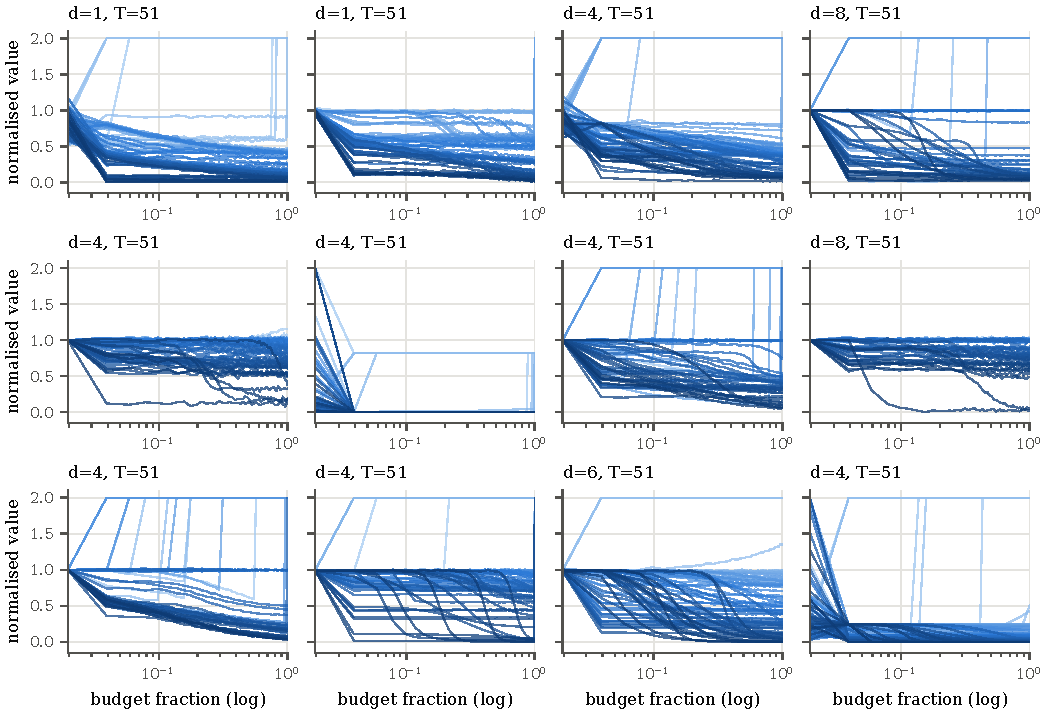
\includegraphics[width=\linewidth]{figures/bpl_gallery.pdf}
  \caption{Twelve tasks generated by \bpl{} (80 random configurations each; colour: final value, dark = good;
  normalised values).}
\end{figure}

\end{document}
